\subsection{ Introducció a la Formula Student }
{
    La Formula Student és una sèrie de competicions automovilístiques en la que
    participen equips formats per estudiants universitaris arran el món. La
    competició consisteix a dissenyar i construir un vehicle monoplaça, i té
    com objectiu final promoure l'excelència entre els estudiants d'enginyeria.
    D'aquesta manera no es valoren només els resultats esportius, sino també
    les capacitats tècniques, la justificació del disseny i la viabilitat
    empresarial de la proposta de negoci que s'elabora de forma paral·lela.

    \begin{figure}[!htb]
        \centering
        \captionsetup{justification=centering,margin=1.5cm}
        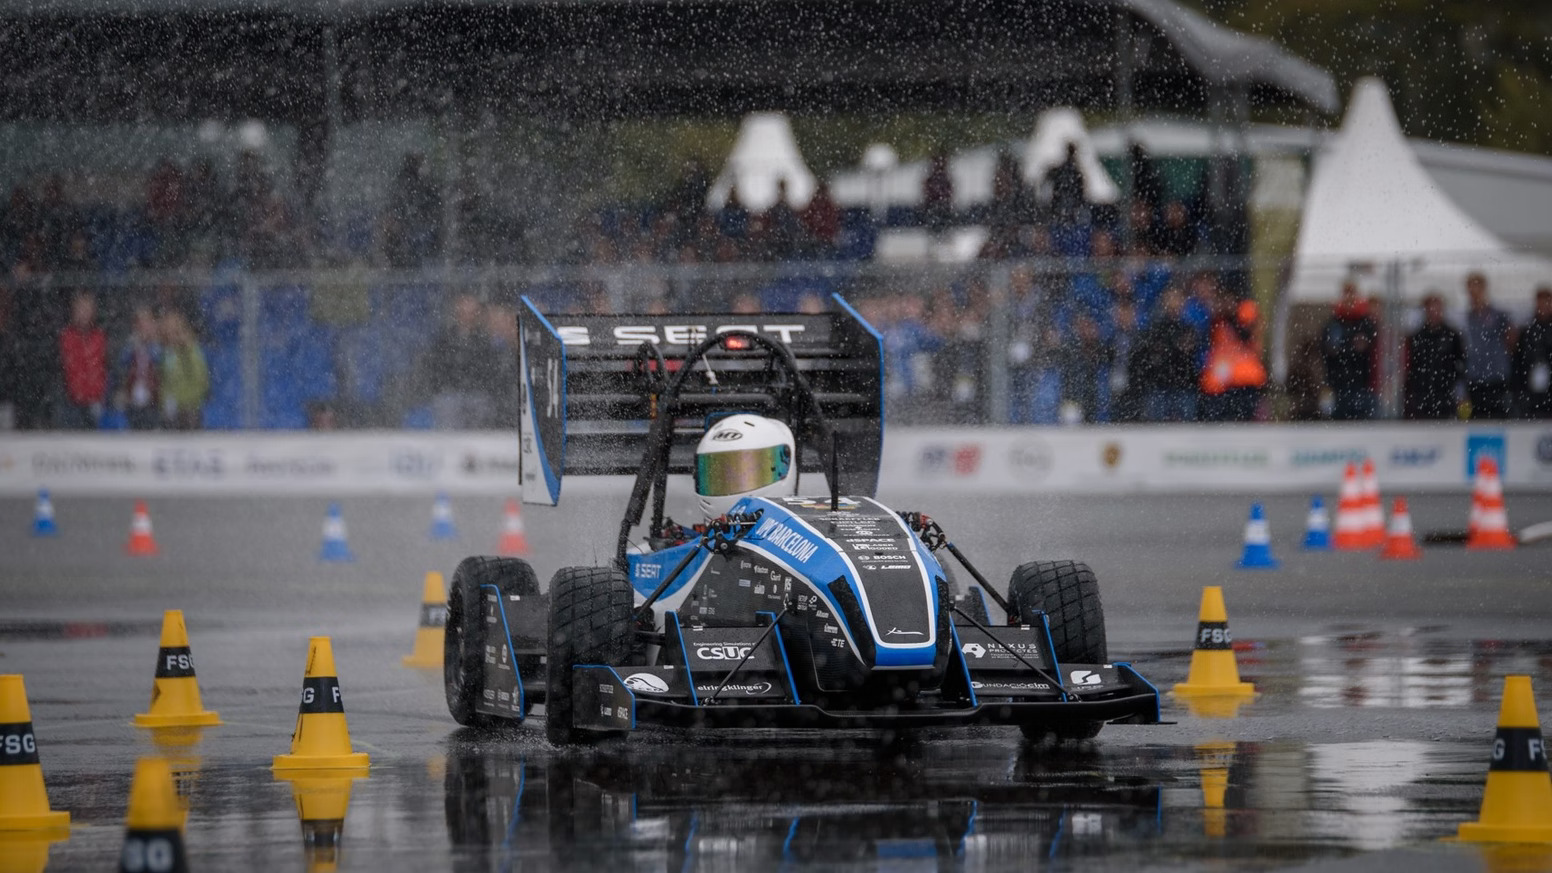
\includegraphics[width=8cm]
            { img/2_formula_student/foto_guay.jpg } 
        \caption[Competició de Formula Student. \emph{BCN eMototsport}]
        { 
            Vehicle de l'equip BCN eMotorsport durant una prova de
            Formula Student. \emph{BCN eMototsport} 
        }
    \end{figure}
    
    La Formula Student va néixer el 1979 de la mà de Mark Marshek, docent de la
    Universitat de Houston, quan va presentar la idea de realitzar competicions
    universitàries d'enginyeria al departament de Relacions Educatives de la
    \ac{SAE}. Poc després, al 1981, es va realitzar la primera edició de la
    Formula \ac{SAE}, en la qual participaren 6 equips formats per uns 40
    estudiants.\cite{formula_student}

    La Formula Student ha anat adaptant-se als avenços tecnològics de les
    últimes dècades. Així, el 2010 es va començar a introduir la mobilitat
    elèctrica, incorporant-se a la competició com una nova categoria. D'altra
    banda, el 2016 es va crear la categoria \emph{Driverless} per donar cabuda
    al desenvolupament de la tecnologia de conducció autònoma.

    Actualment, existeixen més de 700 equips de Formula Student que participen
    en els 17 esdeveniments de Formula Student que tenen lloc al voltant del
    món.
}

\subsection{ BCN eMotorsport }
{
    BCN eMotorsport és l'equip que representa les escoles d'enginyeria de
    l'\ac{ETSEIB} i l'\ac{ETSETB} a les competicions de Formula Student. Cada
    any l'equip dissenya, fabrica i testeja un vehicle monoplaça de competició.

    L'equip és fundat el 2007 per 13 estudiants de l'\ac{ETSEIB}, adoptant el
    nom de \emph{\ac{ETSEIB} Motorsport} i convertint-se en un dels primers
    equips de Formula Student d'Espanya. En aquell precís moment els seus
    membres comencen a treballar en el prototip del seu primer vehicle, el
    CAT01, de combustió interna. L'any 2008 \emph{\ac{ETSEIB} Motorsport}
    participa en la seva primera competició de Formula Student. El 2011,
    l'equip va començar a competir en categoria elèctrica, sent el primer equip
    espanyol en fer-ho. Tots els vehicles posteriors han continuat sent
    elèctrics.

    D'altra banda, l'any 2018 sorgeix un nou projecte a l'\ac{ETSETB} el primer
    equip espanyol en participar en categoria autònoma, \emph{Driverless UPC}.
    Dos anys després, al 2020, es produeix la fusió dels equips de
    \emph{\ac{ETSEIB} Motorsport} i \emph{Driverless UPC}, donant lloc a
    l'equip actual de \emph{BCN eMotorsport}. \cite{bcn_emotorsport}

    Any rere any l'equip afegeix innovacions tècniques per millorar el
    rendiment del vehicle i els resultats a les competicions, entre altres, la
    implementació de l'algorisme de Torque Vectoring per la tracció a quatre
    rodes, la incorporació de frenada regenerativa o un algorisme de State of
    Charge per estimar el nivell de bateria. Aquest any l'equip compleix 15
    anys i uns dels projectes que ha pres més força és el projecte de
    l'inversor propi.

    \begin{figure}[!htb]
        \centering
        \begin{minipage}[c]{7cm}
            \centering
            \captionsetup{justification=centering}
            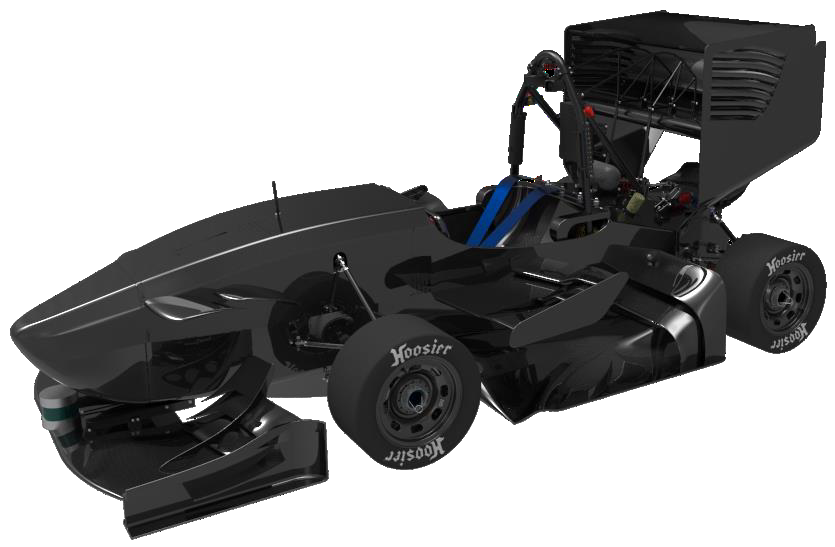
\includegraphics[width=7cm]
                { img/2_formula_student/cat14-x.png }
            \caption[Renderització del CAT14x. \emph{BCN eMotorsport} ]
            { 
                Renderització del vehicle de competició CAT14x d'aquesta
                temporada 2022. \emph{BCN eMotorsport.} 
            }             
        \end{minipage} \hfil
        \begin{minipage}[c]{7cm}
            \centering
            \captionsetup{justification=centering}
            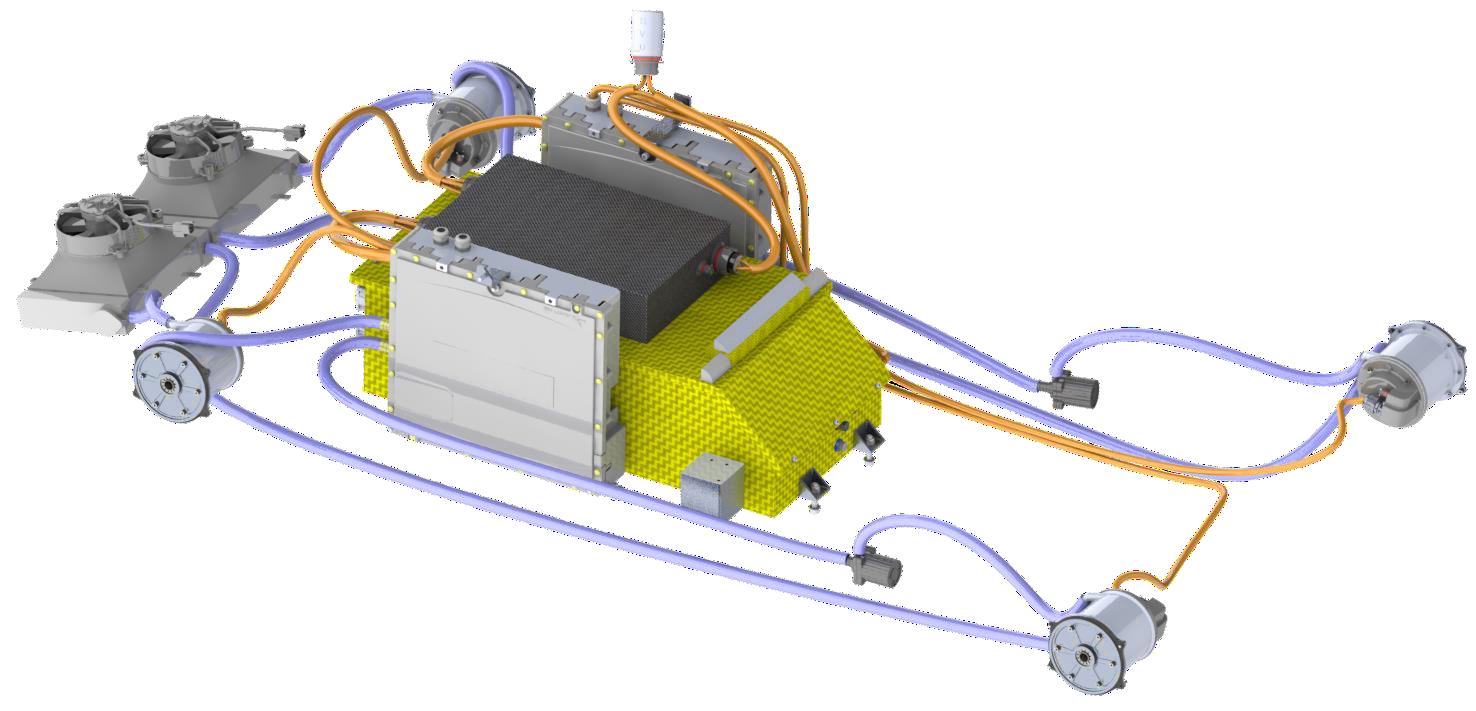
\includegraphics[width=7cm]
                { img/2_formula_student/power.png }
            \caption[Renderització del tren de potència. \emph{BCN eMotorsport} ]
            { 
                Renderització del model en SolidWorks del tren de potència.
                \emph{BCN eMotorsport.}  
            }                
        \end{minipage} \hfil
    \end{figure} 

    Els membres de l'equip es reparteixen en vuit seccions: aerodinàmica,
    chasis, control del vehicle, dinàmica del vehicle, percepció, electrònica,
    gestió i tren de potència. Cada una de les seccions s'encarrega del
    disseny, construcció i testeig d'una part del vehicle, a excepció de
    gestió, que s'encarrega d'elaborar el pla de negoci i gestionar el
    pressupost de l'equip.
}

\subsection{ Introducció al tren de potència }
{
    \begin{figure}[!htb]
        \centering
        \captionsetup{justification=centering, margin=1.5cm}
        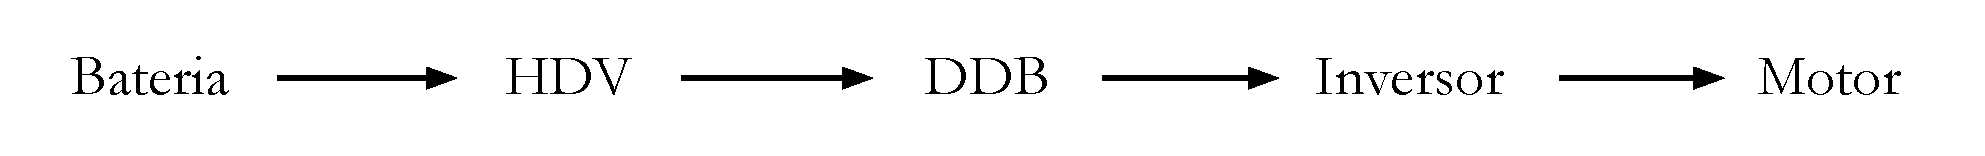
\includegraphics[width=13cm]
            { img/2_formula_student/power.pdf }
        \caption{ Esquema de connexió del tren de potència }
    \end{figure}

    El tren de potència d'un vehicle és el sistema encarregat d'emmagatzemar,
    transformar i entregar l'energia necessària per permetre la seva propulsió.
    En el cas d'un vehicle elèctric, aquest elements són la bateria, el motor,
    l'inversor, el cablejat i altres elements de seguretat. En els succesius
    vehicles elèctrics de l'equip, el tren de potència ha suposat habitualment
    entre el 45\% i el 50\% del seu pes, sent la bateria el component més
    pesat.

    \subsubsection{ Bateria }
    {
        Per reglament de la Formula Student, el voltatge màxim permès és de 600
        V \cite{fs_rules}. La capacitat de la bateria es dimensiona estudiant
        el consum d'energia del vehicle durant la prova de resistència
        (\emph{Endurance}), en la que el vehicle ha de recòrrer una distància
        de 22 km sense carregar les bateries \cite{sergio}. Compta amb un
        sistema de balanceig passiu per mitjà del \ac{BMS} i un circuit de
        precàrrega dels que limita el corrent durant la precàrrega dels
        condensadors de l'inversor, amb el qual és necessari communicar-se
        mitjançant CAN. Les especificacions de la bateria es recullen a la
        taula \ref{bateria}.

        \begin{figure}[!htb]
            \centering
            \captionsetup{justification=centering, margin=1.5cm}
            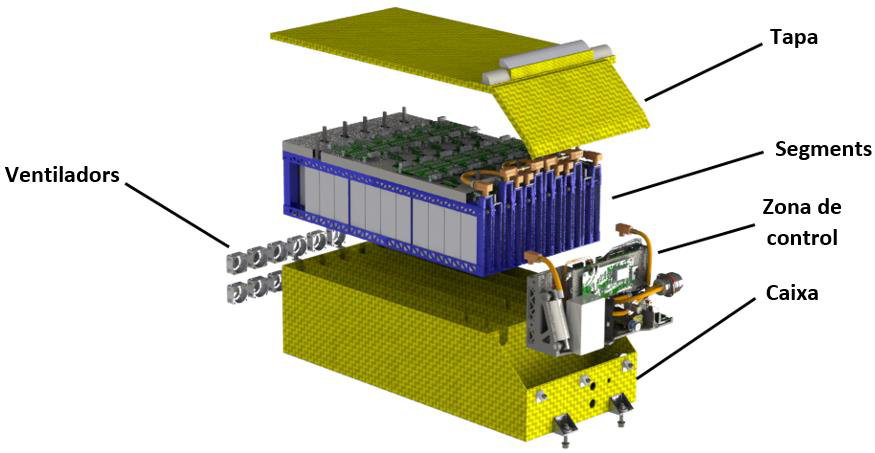
\includegraphics[width=9cm]
                { img/2_formula_student/bateria.png }
            \caption{ Bateria del CAT14x. \emph{BCN eMotorsport.}}
        \end{figure}

        \begin{table}[!htb]
            \caption{ Especificacions de la bateria del CAT14x }
            \label{bateria}
            \centering
            \renewcommand{\arraystretch}{1.3}
            \tablefirsthead{}
            \tablehead{}
            \tabletail{}
            \tablelasttail{}
        
            \begin{tabular}{|l|c|c|}
                \hline
                    \textbf{ Especificació } & 
                    \textbf{ Valor nominal } &
                    \textbf{ Valor màxim } \\
                \hhline{|=|=|=|}
                    { Voltatge total } & 
                        { $525,4 V$ } & 
                        { $596,4\ V$ } \\
                \hline
                    { Energia total } & 
                        { $7145,44\ Wh$ } & 
                        { $8111,04\ Wh$ } \\
                \hline
                    { Potència total } & 
                        { $15,4\ kW$ } & 
                        { $35,366\ kW$ } \\
                \hhline{|=|=|=|}
                    { Disposició de cel·les } & 
                        \multicolumn{2}{|c|}{ $142s2p$ } \\
                \hline
                    { Capacitat total } & 
                        \multicolumn{2}{|c|}{ $13,6\ Ah$ } \\
                \hline
                    { Pes } & 
                        \multicolumn{2}{|c|}{ $35,5\ kg$ } \\
                \hline
            \end{tabular}
        \end{table}
    }

    \subsubsection{ Motor }
    {
        Coneixem com motor elèctric aquell dispisitu capaç de convertir
        l'energia elèctrica en energia mecànica per mitjà de l'interacció
        d'elements capaços de generar i interactuar amb camps magnètics, com
        són els inductors i els imants. Un motor generalment consta de dues
        parts principals, l'estàtor i el rotor, que són la part fixa i la
        rotativa, respectivament. Entre els motors existents podem trobar
        motors que funcionen en continua o en alterna de tres fases o més;
        aquests últims, poden ser alhora síncrons o asíncrons (si la seva
        freqüència de rotació coincideix amb la freqüència de l'ona elèctrica
        que l'alimenta).
    
        El motor utilitzat per l'equip és un motor trifàsic síncron d'imants
        permanents interiors (\acs{IPMSM}). Aquest tipus de motor es
        carateritza per incorporar imants a l'interior del rotor, a diferència
        dels SPMSM, que els porten a la superfície del rotor. Els motors
        \acs{PMSM} són motors que admeten una densitat de potència molt
        elevada, en relació amb el seu pes i dimensions. A sobre, els motors
        IPMSM tenen una eficiencia una mica superior als SPMSM en aprofitar el
        parell de reluctància i poden assolir velocitats majors degut a que la
        tècnica de debilitament de camp (FW) és més apropiada amb imants
        permanents.

        \begin{figure}[!htb]
            \centering
            \captionsetup{justification=centering, margin=1.5cm}
            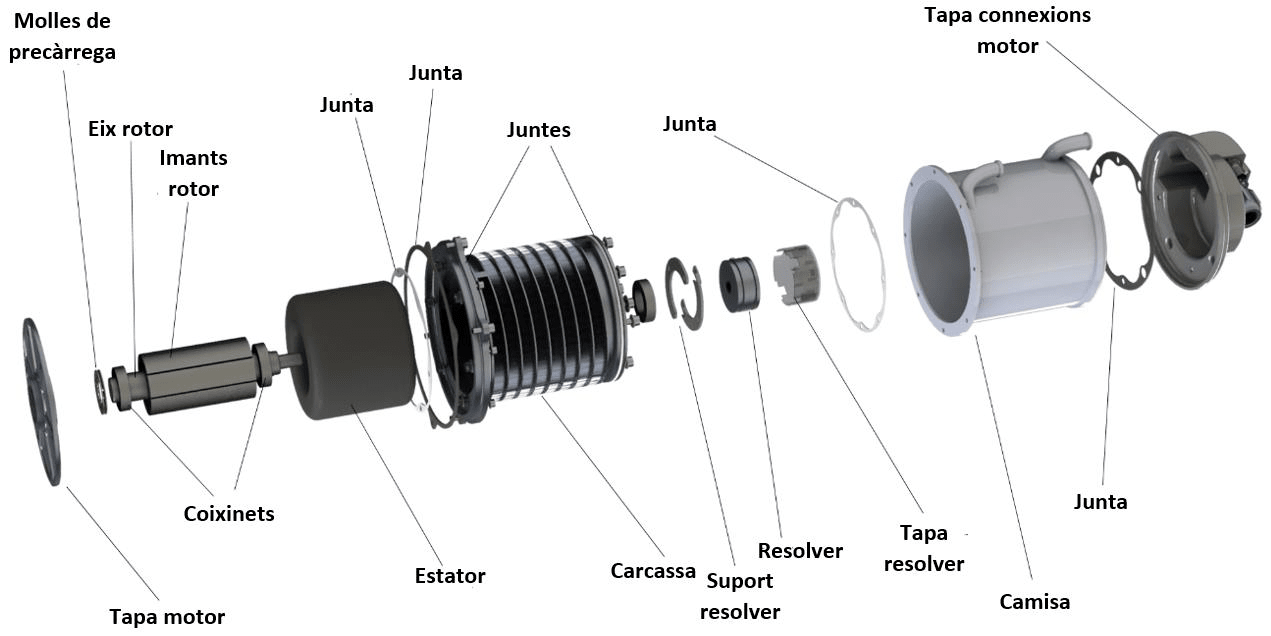
\includegraphics[width=10cm]
                { img/2_formula_student/motor.png }
            \caption{ Vista explosionada del motor del CAT14x. \emph{BCN eMotorsport.}}
        \end{figure}

        \begin{table}[!htb]
            \caption{ Fitxa tècnica del motor Fischer TI085-052-070-04B7S-07S04BE2 }
            \label{motor}
            \centering
            \renewcommand{\arraystretch}{1.3}
            \tablefirsthead{}
            \tablehead{}
            \tabletail{}
            \tablelasttail{}
        
            \begin{tabular}{|l|c|c|}
                \hline
                    \textbf{ Especificació } & 
                    \textbf{ Valor nominal } &
                    \textbf{ Valor màxim } \\
                \hhline{|=|=|=|}
                    { Parell } & 
                    { $11,1\ Nm$ } & 
                    { $29,1\ Nm$ } \\
                \hline
                    { Corrent eficaç } & 
                    { $22,6\ A_{rms}$ } & 
                    { $29,1\ A_{rms}$ } \\
                \hline
                    { Velocitat angular } & 
                    { $13250\ rpm$ } & 
                    { $20000\ rpm$ } \\
                \hline
                    { Potència } & 
                    { $15,4\ kW$ } & 
                    { $35,366\ kW$ } \\
                \hhline{|=|=|=|}
                    { Voltatge bus DC } & 
                    \multicolumn{2}{|c|}{ $600\ V$ } \\
                \hline
                    { Número de parells de pols } & 
                    \multicolumn{2}{|c|}{ 4 } \\
                \hline
                    { Resistència } & 
                    \multicolumn{2}{|c|}{ $0,126\ \Omega$ } \\
                \hline
                    { Inductància } & 
                    \multicolumn{2}{|c|}{ $0,393\ mH$ } \\
                \hline
                    { Tipus de connexió } & 
                    \multicolumn{2}{|c|}{ Estrella } \\
                \hline
                    { Velocitat al parell màxim } & 
                    \multicolumn{2}{|c|}{ $11600\ rpm$ } \\
                \hline
                    { Pes } & 
                    \multicolumn{2}{|c|}{ $4,5\ kg$ } \\
                \hline
            \end{tabular}
        \end{table}

        El CAT14x incorpora quatre motors IPMSM comercials de la marca
        \emph{Fischer Elektromotoren}, les especificacions del qual es
        resumeixen en la taula \ref{motor}. Disposar de quatre motors permet
        tenir tracció a quatre rodes (\emph{Four-wheel drive} o 4WD), la qual
        està controlada computacionalment per un algorisme de \emph{Torque
        Vectoring} desenvolupat per l'equip i implementat en la unitat de
        processament (\emph{Processing Unit}, PU) del vehicle.

        La mesura de l'angle del rotor respecte a l'estàtor es realitza
        actualment per mitjà de resolver. Es va barajar la idea de canviar d'un
        resolver a un encoder, però es decidí finalment continuar amb el
        resolver. Els resolvers són en general molt més robustos davant EMIs,
        ja que no disposen d'elements electrònics. No obstant, requereixen d'un
        circuit d'adequació, en el qual s'implementen amplificadors de senyal i
        algún sistema de detecció de l'angle i la velocitat angular, com
        pot ser un PLL (\emph{Phase Loocked Loop}). No obstant això, el
        requisit de fer intercanviable el nou inversor amb l'actual ha decantat
        la balança a favor del resolver.
    }

    \subsubsection{ Inversor }
    {
        Es coneix generalment com inversor, inversor de potència o ondulador al
        dispositiu encarregat de transferir potència d'una font de tensió
        continua a una càrrega de alterna. En el cas del vehicle de FS, la
        potència de la bateria es transfereix a cada un dels quatre motors per
        mitjà d'inversors.

        Els inversors que es fan servir per controlar la velocitat, el torque
        i/o la posició d'un motor es coneixen a la literatura com \emph{Motor
        Drive} (``conducció de motor''). En aquests casos es considera l'inversor
        com un component del \emph{Motor Drive}, en conjunció al motor, el
        sistema de control electrònic i els diversos sensors que tanquen el
        llaç de control.

        Els \emph{Motor Drives} que porta el vehicle d'aquesta temporada 2022,
        el CAT14x, són els doble inversors Lenze Mobile DSU 60/60, que porten
        dos inversors cadascun \cite{lenze}. Aquests inversors estan
        inicialment concebuts per la seva implementació en autobusos de tracció
        elèctrica i altres vehicles semblants destinats a la movilitat urbana.
        Es pot deduir, per tant, que es troba sobredimensionat per a la nostra
        aplicació particular d'un vehicle de competició que no sobrepassa els
        250 kg i està limitat a 80 kW de potència total per reglament
        \cite{fs_rules}.

        \begin{figure}[!htb]
            \centering
            \begin{minipage}[c]{7cm}
                \centering
                \captionsetup{justification=centering}
                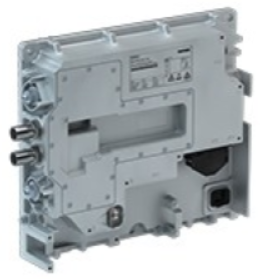
\includegraphics[width=5cm]
                { img/2_formula_student/inverter.png }
                \caption{ Doble inversor Lenze Mobile DSU 60/60. }
            \end{minipage} \hfil
            \begin{minipage}[c]{7cm}
                \centering
                \captionsetup{justification=centering}
                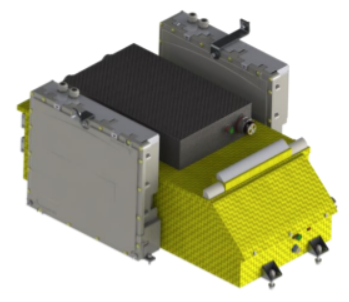
\includegraphics[width=5cm]
                { img/2_formula_student/inverter2.png } 
                \caption[ Col·locació dels Lenze Mobile ]
                { 
                    Col·locació dels dos Lenze Mobile DSU 60/60 respecte la
                    resta del tren de potència. \emph{BCN eMotorsport}
                }
            \end{minipage} \hfil
        \end{figure}

        \begin{table}[!htb]
            \caption{ Fitxa tècnica del doble inversor Lenze Mobile DSU 60/60 }
            \centering
            \renewcommand{\arraystretch}{1.3}
            \tablefirsthead{}
            \tablehead{}
            \tabletail{}
            \tablelasttail{}
        
            \begin{tabular}{|m{4cm}|c|c|c|}
                \hline
                    \textbf{ Especificació } & 
                    \textbf{ Mínima } &
                    \textbf{ Nominal } &
                    \textbf{ Màxima } \\
                \hhline{|=|=|=|=|}
                    { Voltatge bus DC } &
                    { $100\ V$ } &
                    { $800\ V$ } &
                    { $848\ V$ } \\
                \hline
                    { Tensió de sortida per fase } & 
                    { $0\ V$ } &
                    { - } & 
                    { $510\ V$ } \\
                \hline
                    { Freqüència de sortida } & 
                    { $-599\ Hz$ } & 
                    { - } & 
                    { $599\ Hz$ } \\
                \hline
                    { Corrent de curtcircuit a l'apagada } & 
                    { - } & 
                    { $96,2\ A$ } &
                    { - } \\
                \hline
                    { Consum de corrent } & 
                    { - } & 
                    { $39,2\ A$ } & 
                    { $70,5\ A$ } \\
                \hline
                    { Potència de sortida } & 
                    { - } & 
                    { $20\ kW$ } & 
                    { $36\ kW$ } \\
                \hline
                    { Corrent de sortida (segons conmutació) } & 
                    { $16\ A\ (16\ kHz)$ } & 
                    { $28,8\ A\ (8\ kHz)$ } &                    
                    { $51,2\ A\ (2\ kHz)$ } \\
                \hhline{|=|=|=|=|}
                    { Pes } & 
                    \multicolumn{3}{|c|}{ $7,4\ kg$ } \\
                \hline
                    { Dimensions } & 
                    \multicolumn{3}{|c|}{ $310,6 mm \times 354,5 mm \times 75 mm$ } \\
                \hline
            \end{tabular}
        \end{table}

        El projecte de l'inversor propi apareix com alternativa a l'inversor
        Lenze Mobile DSU 60/60. Com s'ha comentat, l'inversor es troba
        sobredimensionat respecte les característiques del vehicle; no obstant,
        aquest no és l'únic desavantatge. 
        
        Tenim per un costat que el funcionament intern dels Lenze és totalment
        desconegut per l'equip. El fabricant aporta documentació respecte a
        l'interfície de comunicació i els modes de funcionament, però no acaba
        d'explicar com aprofitar el rendiment de l'inversor. 
        
        Per l'altre costat, el fabricant ha imposat un límit en quan a la
        freqüència amb la qual es poden enviar i rebre comandes pel bus CAN
        (uns 50 Hz). Aquesta limitació no permet estudiar amb profunditat el
        rendiment de l'inversor en els diferents test que es realitzen a
        bancada i actualment s'hi dedica bastant de temp a ajustar
        artesanalment els controladors de corrent, a falta d'un millor equip
        d'instrumentació (torquímetres o generadors de mapes d'eficiència,
        entre altres).

        Respecte a les especificacions del nou inversor, cal mencionar el pas a
        tecnologia de transistor MOSFET \ac{SiC}, que permeten una freqüència
        de commutació més elevada que els IGBT de l'inversor actual. En afegit,
        es preveu que la carcassa protectora (\emph{housing}) del nou inversor
        reduexi significativament el pes d'aquest component. Malgrat això,
        segueix sent un projecte bastant arriscat i costós.
    } 

    \subsubsection{ Altres elements del tren de potència }
    {
        Els elements del tren de potència que no han set explicats encara són el
        \ac{HVD}, la \ac{DDB} i el cablejat:

        \begin{itemize}
            \item \textbf{\Acl{HVD}:} 
                És un element de seguretat que funciona com un interruptor amb el
                que s'obre el circuit d'alt voltatge i el de seguretat. 

            \item \textbf{\Acl{DDB}:}
                És una capsa en la que es troben components de recolecció de
                dades sobre l'estat del circuit d'alt voltatge i de
                distribució. La funció del circuit de distribució és bifurcar
                en quatre branques, un per cada motor, el bus DC que prové de
                la bateria. En la \ac{DDB} també es troba el circuit de
                descàrrega dels condensadors de l'inversor.

                \begin{figure}[!htb]
                    \centering
                    \begin{minipage}[c]{7cm}
                        \centering
                        \captionsetup{justification=centering}
                        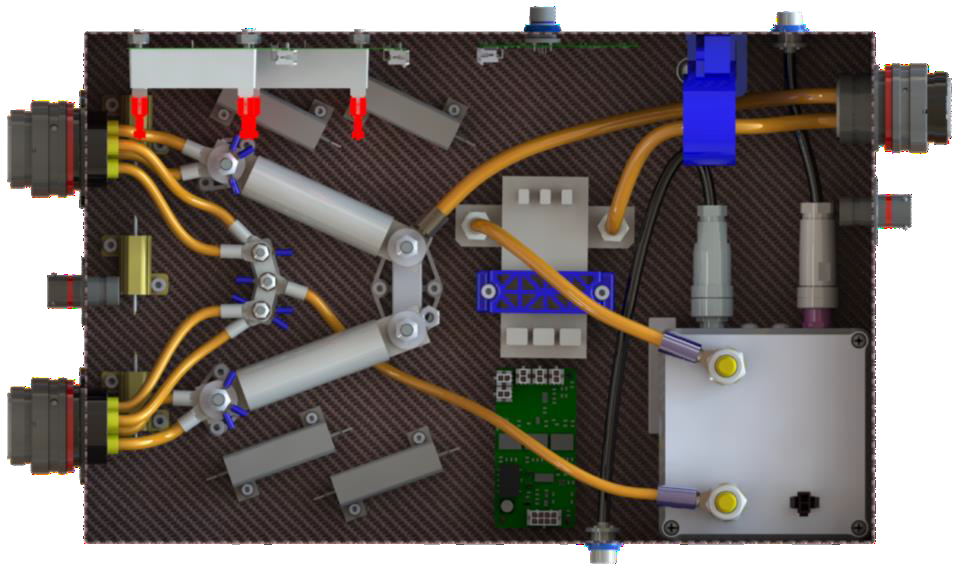
\includegraphics[width=7cm]
                            { img/2_formula_student/ddb.png }
                        \caption{Data and distribution box. \emph{BCN eMotorsport}}             
                    \end{minipage} \hfil
                    \begin{minipage}[c]{7cm}
                        \centering
                        \captionsetup{justification=centering}
                        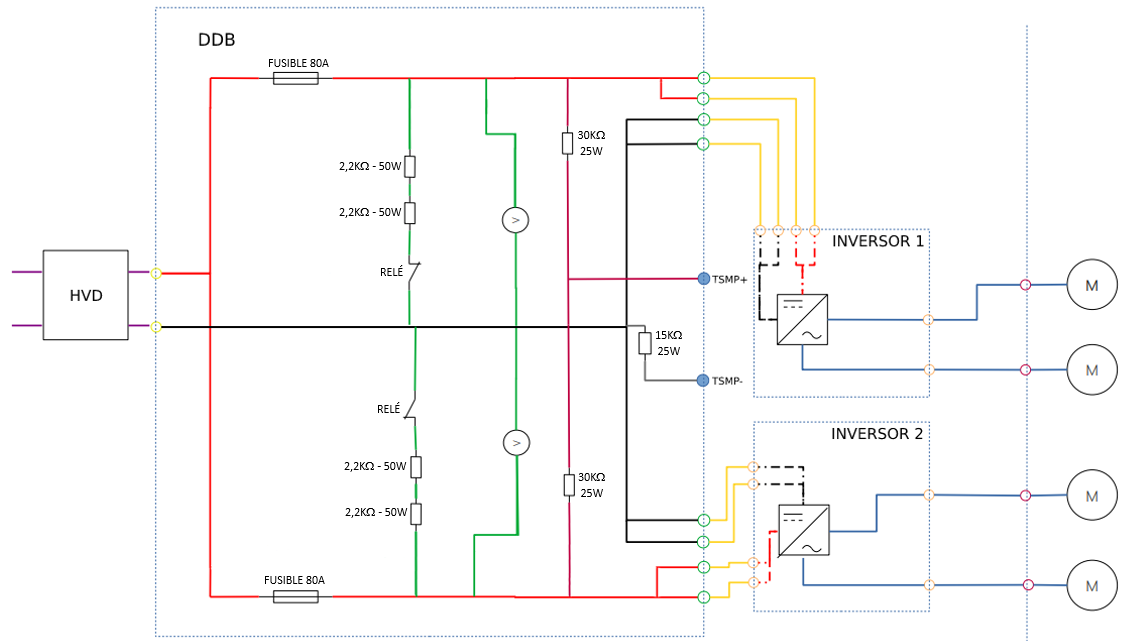
\includegraphics[width=7cm]
                            { img/2_formula_student/circuit.png }
                        \caption{Circuit de distribució. \emph{BCN eMotorsport}}                
                    \end{minipage} \hfil
                \end{figure}

            \item \textbf{Cablejat:}
                Pel cablejat del circuit d'alt voltatge es fa servir cablejat
                blindat Radox de la marca Huber\&Suhner. Per normativa, el
                cablejat ha de ser de color taronja \cite{fs_rules}.
        \end{itemize}
    }
}